\def\filename{Rozdział 3}

\chapter{Próba symulacji wyborów na podstawie wyników z~2019 roku}

\section{Obróbka danych z~PKW}
W celu przeprowadzenia symulacji niezbędne było posiadanie odpowiednich danych z~wynikami wyborów do Sejmu z~2019 roku z~Państwowej Komisji Wyborczej. Ze względu na konieczność przypisania wyników do zupełnie nowych okręgów wyborczych, gdzie w~przypadku dużych miast dzielone były nawet osiedla, czy dzielnice, niezbędne były wyniki z~uwzględnieniem pojedynczych obwodów.

Ponieważ nie istniał żaden arkusz danych zawierający podział Polski na zupełnie nowe okręgi, taki arkusz należało przygotować samodzielnie. W tym celu na podstawie projektu ustawy Fundacji im. Madisona oraz listy obwodów ze strony PKW utworzyłem plik z~nowym podziałem według zasady jeden arkusz to jeden okręg. W pliku znajdują się wyłącznie unikalne kody danego obwodu wraz nazwą gminy/miasta na prawach powiatu na terenie którego się znajduje.
Następnie poprzez przypisanie liczby głosów oddanych na konkretne komitety wyborcze w~każdym obwodzie, jesteśmy w~stanie je zsumować oraz określić, który komitet zdobył największą liczbę głosów w~każdym okręgu.


\begin{table}[]
\caption{Wyniki wyborów w~obwodach miasta Bolesławiec (wybrane kolumny)}
\centering
\begin{adjustbox}{angle=90}
\scalebox{0.6}{
\begin{tabular}{|l|l|l|l|l|l|l|l|l|l|l|l|l|l|l|l|l|l|l|}
\hline
symbol                                  & TERYT  & Okręg & numer & Typ\_obszar & Gmina          & Powiat        & Woj.         & Głosy & ko  & Emeryci & Konf & PSL & Prawica & PIS & Liroy & SLD & BIS & Niemcy \\ \hline
6a18-a07e-c240-e60e-2b2c-d9ee-4b6f-30b6 & 020101 & 1     & 1     & miasto      & m. Bolesławiec & bolesławiecki & dolnośląskie & 882   & 202 &         & 72   & 46  &         & 368 &       & 145 & 49  &        \\ \hline
87e0-d41a-ce4f-cde5-c934-67c7-4577-0bdd & 020101 & 1     & 2     & miasto      & m. Bolesławiec & bolesławiecki & dolnośląskie & 870   & 223 &         & 57   & 41  &         & 307 &       & 196 & 46  &        \\ \hline
ec4f-7f57-b0eb-d14d-85b3-0095-8b38-265c & 020101 & 1     & 3     & miasto      & m. Bolesławiec & bolesławiecki & dolnośląskie & 893   & 193 &         & 55   & 52  &         & 331 &       & 194 & 68  &        \\ \hline
5440-a0cd-5860-fdab-0a77-7c24-e35d-da10 & 020101 & 1     & 4     & miasto      & m. Bolesławiec & bolesławiecki & dolnośląskie & 945   & 234 &         & 65   & 53  &         & 355 &       & 191 & 47  &        \\ \hline
1ff9-1ec2-d664-fc91-5eee-71b7-d300-904e & 020101 & 1     & 5     & miasto      & m. Bolesławiec & bolesławiecki & dolnośląskie & 819   & 215 &         & 33   & 54  &         & 288 &       & 176 & 53  &        \\ \hline
9b86-97d7-7785-87ee-564e-72df-8e49-6623 & 020101 & 1     & 6     & miasto      & m. Bolesławiec & bolesławiecki & dolnośląskie & 624   & 126 &         & 31   & 45  &         & 243 &       & 136 & 43  &        \\ \hline
bd9b-6fa6-8202-a10b-73dc-b3c0-0116-1c25 & 020101 & 1     & 7     & miasto      & m. Bolesławiec & bolesławiecki & dolnośląskie & 881   & 219 &         & 37   & 35  &         & 309 &       & 216 & 65  &        \\ \hline
6d4e-9db8-11ff-e061-e722-a052-a5fb-986b & 020101 & 1     & 8     & miasto      & m. Bolesławiec & bolesławiecki & dolnośląskie & 934   & 202 &         & 59   & 61  &         & 349 &       & 196 & 67  &        \\ \hline
559e-dcef-df28-04be-601e-c7eb-e0e8-e537 & 020101 & 1     & 9     & miasto      & m. Bolesławiec & bolesławiecki & dolnośląskie & 856   & 218 &         & 39   & 42  &         & 298 &       & 205 & 54  &        \\ \hline
49b7-93ae-a838-a030-5ae5-0763-3a97-80d8 & 020101 & 1     & 10    & miasto      & m. Bolesławiec & bolesławiecki & dolnośląskie & 744   & 141 &         & 40   & 32  &         & 296 &       & 174 & 61  &        \\ \hline
fbee-2d88-0e69-c176-5eab-683a-be67-7268 & 020101 & 1     & 11    & miasto      & m. Bolesławiec & bolesławiecki & dolnośląskie & 830   & 189 &         & 52   & 45  &         & 275 &       & 218 & 51  &        \\ \hline
1c5a-0422-f533-9b92-f0e2-b7eb-812c-fe87 & 020101 & 1     & 12    & miasto      & m. Bolesławiec & bolesławiecki & dolnośląskie & 804   & 182 &         & 36   & 35  &         & 321 &       & 192 & 38  &        \\ \hline
9025-36e7-13d1-6852-f28a-71b8-67c6-b044 & 020101 & 1     & 13    & miasto      & m. Bolesławiec & bolesławiecki & dolnośląskie & 821   & 192 &         & 45   & 40  &         & 293 &       & 189 & 62  &        \\ \hline
1c63-4523-2475-6dd6-bf8f-7a82-9b7c-a745 & 020101 & 1     & 14    & miasto      & m. Bolesławiec & bolesławiecki & dolnośląskie & 973   & 250 &         & 61   & 53  &         & 320 &       & 242 & 47  &        \\ \hline
dfab-8b60-54a2-1752-1f43-2dac-0cff-691e & 020101 & 1     & 15    & miasto      & m. Bolesławiec & bolesławiecki & dolnośląskie & 914   & 243 &         & 40   & 36  &         & 311 &       & 232 & 52  &        \\ \hline
dcb6-2b21-cae0-1280-53ef-492a-2fd8-7c5d & 020101 & 1     & 16    & miasto      & m. Bolesławiec & bolesławiecki & dolnośląskie & 901   & 213 &         & 65   & 55  &         & 292 &       & 228 & 48  &        \\ \hline
6717-b552-d9a0-0081-66c6-2156-273f-620d & 020101 & 1     & 17    & miasto      & m. Bolesławiec & bolesławiecki & dolnośląskie & 658   & 133 &         & 53   & 31  &         & 255 &       & 145 & 41  &        \\ \hline
e4aa-8a1a-1692-e727-9b11-f740-a017-8df2 & 020101 & 1     & 18    & miasto      & m. Bolesławiec & bolesławiecki & dolnośląskie & 699   & 150 &         & 62   & 41  &         & 258 &       & 146 & 42  &        \\ \hline
17b8-7a98-18f8-140b-dc73-5381-bab7-d77b & 020101 & 1     & 19    & miasto      & m. Bolesławiec & bolesławiecki & dolnośląskie & 972   & 314 &         & 57   & 62  &         & 265 &       & 204 & 70  &        \\ \hline
45cc-1e2a-8f6c-7c49-c7e0-c191-dc42-25d9 & 020101 & 1     & 20    & miasto      & m. Bolesławiec & bolesławiecki & dolnośląskie & 962   & 228 &         & 88   & 55  &         & 335 &       & 178 & 78  &        \\ \hline
c8f8-30e1-f88f-aa6d-0a4f-b2e1-dfa1-564c & 020101 & 1     & 21    & miasto      & m. Bolesławiec & bolesławiecki & dolnośląskie & 889   & 216 &         & 58   & 44  &         & 320 &       & 185 & 66  &        \\ \hline
eb54-5f02-bd32-af84-ff5f-2128-82e1-68e5 & 020101 & 1     & 22    & miasto      & m. Bolesławiec & bolesławiecki & dolnośląskie & 26    & 6   &         & 2    & 2   &         & 11  &       & 5   & 0   &        \\ \hline
cc5c-dc47-3427-1558-3871-803e-ed80-b91c & 020101 & 1     & 23    & miasto      & m. Bolesławiec & bolesławiecki & dolnośląskie & 60    & 10  &         & 1    & 10  &         & 33  &       & 4   & 2   &        \\ \hline
caec-17c3-1064-2e4f-900e-1e7c-a195-4f6c & 020101 & 1     & 24    & miasto      & m. Bolesławiec & bolesławiecki & dolnośląskie & 32    & 9   &         & 1    & 2   &         & 12  &       & 0   & 8   &        \\ \hline
\end{tabular}}
\end{adjustbox}
\caption*{Źródło: \url{sejmsenat2019.pkw.gov.pl}}
\end{table}

\begin{table}[]
\caption{Obwody okręgu 3 (Bolesławiec) w~nowym podziale na JOW}
\centering
\scalebox{0.7}{
\begin{tabular}{|l|l|}
\hline
Symbol & Opis \\ \hline
6a18-a07e-c240-e60e-2b2c-d9ee-4b6f-30b6 & m. Bolesławiec \\ \hline
87e0-d41a-ce4f-cde5-c934-67c7-4577-0bdd & m. Bolesławiec \\ \hline
ec4f-7f57-b0eb-d14d-85b3-0095-8b38-265c & m. Bolesławiec \\ \hline
5440-a0cd-5860-fdab-0a77-7c24-e35d-da10 & m. Bolesławiec \\ \hline
1ff9-1ec2-d664-fc91-5eee-71b7-d300-904e & m. Bolesławiec \\ \hline
9b86-97d7-7785-87ee-564e-72df-8e49-6623 & m. Bolesławiec \\ \hline
bd9b-6fa6-8202-a10b-73dc-b3c0-0116-1c25 & m. Bolesławiec \\ \hline
6d4e-9db8-11ff-e061-e722-a052-a5fb-986b & m. Bolesławiec \\ \hline
559e-dcef-df28-04be-601e-c7eb-e0e8-e537 & m. Bolesławiec \\ \hline
49b7-93ae-a838-a030-5ae5-0763-3a97-80d8 & m. Bolesławiec \\ \hline
fbee-2d88-0e69-c176-5eab-683a-be67-7268 & m. Bolesławiec \\ \hline
1c5a-0422-f533-9b92-f0e2-b7eb-812c-fe87 & m. Bolesławiec \\ \hline
9025-36e7-13d1-6852-f28a-71b8-67c6-b044 & m. Bolesławiec \\ \hline
1c63-4523-2475-6dd6-bf8f-7a82-9b7c-a745 & m. Bolesławiec \\ \hline
dfab-8b60-54a2-1752-1f43-2dac-0cff-691e & m. Bolesławiec \\ \hline
dcb6-2b21-cae0-1280-53ef-492a-2fd8-7c5d & m. Bolesławiec \\ \hline
6717-b552-d9a0-0081-66c6-2156-273f-620d & m. Bolesławiec \\ \hline
e4aa-8a1a-1692-e727-9b11-f740-a017-8df2 & m. Bolesławiec \\ \hline
17b8-7a98-18f8-140b-dc73-5381-bab7-d77b & m. Bolesławiec \\ \hline
45cc-1e2a-8f6c-7c49-c7e0-c191-dc42-25d9 & m. Bolesławiec \\ \hline
c8f8-30e1-f88f-aa6d-0a4f-b2e1-dfa1-564c & m. Bolesławiec \\ \hline
eb54-5f02-bd32-af84-ff5f-2128-82e1-68e5 & m. Bolesławiec \\ \hline
cc5c-dc47-3427-1558-3871-803e-ed80-b91c & m. Bolesławiec \\ \hline
caec-17c3-1064-2e4f-900e-1e7c-a195-4f6c & m. Bolesławiec \\ \hline
5f5f-4cf2-1f4c-d082-efcc-0000-0244-19b6 & gm. Bolesławiec \\ \hline
20a1-7a35-b261-cff2-b20b-4f2b-1ad6-af0c & gm. Bolesławiec \\ \hline
4583-a552-3f9c-2889-4c1a-78a5-0498-73ed & gm. Bolesławiec \\ \hline
471c-225d-49bf-554b-b06b-6799-3733-d64c & gm. Bolesławiec \\ \hline
9522-204f-f7fc-f259-391b-ecda-cdeb-642d & gm. Bolesławiec \\ \hline
43b6-6df9-f79d-146c-6b7c-aab3-734e-7e4a & gm. Bolesławiec \\ \hline
78b4-64b1-345b-9e2b-f536-9da1-60f3-9803 & gm. Bolesławiec \\ \hline
7c57-a44a-1322-439a-5769-4e6f-db8d-b13c & gm. Bolesławiec \\ \hline
4ce9-4ed3-18f8-358c-0cec-ade0-b074-d4e0 & gm. Bolesławiec \\ \hline
7cf0-f142-6369-6d20-ad70-9787-af79-52bd & gm. Bolesławiec \\ \hline
5db4-51dc-481c-6606-9286-8c1e-c72d-3302 & gm. Bolesławiec \\ \hline
2ca1-1511-043e-55ab-c20f-889f-075d-2884 & gm. Gromadka \\ \hline
80a8-bae0-1c3c-4fea-f2ba-8fa2-b1bc-ecb6 & gm. Gromadka \\ \hline
73dd-4cf0-19dd-faaf-8e9a-d486-943f-2f80 & gm. Gromadka \\ \hline
7995-3a75-3871-03d2-a840-13d8-c82c-b6fe & gm. Gromadka \\ \hline
6315-4be6-7775-a184-78c6-fbbc-704c-f14a & gm. Osiecznica \\ \hline
9eae-727b-68e0-feae-2dcd-e8ca-f43c-9940 & gm. Osiecznica \\ \hline
e245-1198-d402-02d9-abed-5eca-8a0d-ff45 & gm. Osiecznica \\ \hline
1cc8-b167-f40b-6609-ed63-ad3e-7359-2f76 & gm. Osiecznica \\ \hline
419f-e6dd-93b3-f775-212b-44d7-fed1-1c5d & gm. Osiecznica \\ \hline
b949-9b69-9630-3f77-836b-a1cb-8ea5-6514 & gm. Osiecznica \\ \hline
9e2f-dc96-fd52-8f37-4ebc-afa2-4887-de28 & gm. Osiecznica \\ \hline
0fc4-a4be-1c1c-1f45-2688-b1b3-0807-ac3a & gm. Warta Bolesławiecka \\ \hline
c8af-b975-8f70-8761-7ab7-7c40-9144-a88d & gm. Warta Bolesławiecka \\ \hline
af10-d9cc-1e81-c8dd-f9a2-7b42-ccc0-170b & gm. Warta Bolesławiecka \\ \hline
42cf-b599-d4ef-1882-4e89-8826-381b-ee6c & gm. Warta Bolesławiecka \\ \hline
706e-2327-033a-84f0-3104-2075-9c9f-7627 & gm. Warta Bolesławiecka \\ \hline
edfe-29d0-7a4c-1071-9caa-494c-b439-6e15 & gm. Warta Bolesławiecka \\ \hline
6378-e8f8-693a-3626-9037-c82d-0a12-18a9 & gm. Przemków \\ \hline
ec7e-321f-67e5-973d-762f-3cc3-468b-7b0a & gm. Przemków \\ \hline
cffd-0b92-a79d-be52-53d9-1656-69b0-a900 & gm. Przemków \\ \hline
a7eb-089c-e9ee-30c9-af41-ebe2-5bd4-ad43 & gm. Przemków \\ \hline
d99a-5dff-f368-88a2-5414-68aa-eb58-af54 & gm. Przemków \\ \hline
ace3-9551-1a4b-794e-660e-13c3-18fa-3503 & gm. Przemków \\ \hline
8401-4ed1-c04f-99f0-79fc-7e85-299b-92a4 & gm. Przemków \\ \hline
\end{tabular}}
\caption*{Źródło: własne}
\end{table}


\section{Wykorzystane pakiety w~programie RStudio}

Ponieważ wszystkie analizowane dane są przechowywane w~plikach programu Microsoft Excel w~formacie
\textit{xlsx} do ich wczytania w~programie RStudio potrzebny był pakiet \textit{readxl}. Do ułatwienia pracy nad wczytanymi obiektami typu \textit{data frame} użyto pakietu \textit{dplyr}.

Do przeprowadzenia wizualizacji wyników na kartogramie z~podziałem administracyjnym Polski na województwa należało użyć następujących pakietów:
\begin{itemize}
        \item \textit{tmap} - pakiet przeznaczony do tworzenia wykresów mapowych, w~tym kartogramów. Jego zasada działania jest podobna do pakietu \textit{ggplot2}, ale jest dostosowana do działania na kartogramach;
        \item  \textit{tmaptools} - paket wspierający działanie pakietu \textit{tmap};
        \item \textit{sf} - pakiet służący do odczytu i~zapisu plików \textit{shape}, potrzebnych do tworzenia własnych kartogramów.
\end{itemize}


Pierwszym czytanym plikiem jest arkusz z~wynikami wyborów po obwodach, zapisany jako obiekt \textit{wyniki}, oraz wyodrębnienie z~niego wyłącznie tych kolumn, które będą potrzebne w~dalszej pracy, tj.: symbol(kod) obwodu, kod TERYT, liczba oddanych głosów oraz wyniki poszczególnych komitetów wyborczych.

\newpage

\section{Przeprowadzenie prognozy w~RStudio}

Ze względu na przeprowadzenie prognozy według dwóch różnych scenariuszy, według pierwszego wyborca miałby zagłosować na któreś z~komitetów wyborczych z~2019 roku oraz drugie gdzie miałby do wyboru dwa duże bloki wyborcze - lewicowy i~prawicowy, należało przygotować dwie wersje kodów w~języku R.

Do zwrócenia informacji, który kandydat danego komitetu (lub hipotetycznego bloku w~scenariuszu II) wygrał wybory w~danym okręgu wyborczym przygotowano funkcje \textit{mandat1()} oraz \textit{mandat2()}. Za pomocą instrukcji \textit{if...else} funkcja zwraca nazwę komitetu (bloku) z~najwyższą liczbą głosów.

\subsection{Scenariusz I}
Pierwszą wykonaną akcją jest utworzenia obiektu \textit{df1}, przechowującego informację jaką sumę głosów w~każdym z~460 okręgów zdobył każdy z~komitetów, do jakiego województwa należy okręg (kod TERYT) oraz który z~komitetów zdobył mandat.

Ponieważ każdy z~460 okręgów ma przechowywane symbole swoich obwodów w~osobnym arkuszu pliku \textit{xlsx} niezbędne jest utworzenie pętli z~460 iteracjami. W każdej iteracji wczytywany za pomocą funkcji \textit{read\textunderscore excel()} jest jeden kolejny okręg z~wcześniej przygotowanego pliku \textit{nowe\textunderscore jow.xlsx} i~zapisywany jako obiekt \textit{okreg}. Do każdego wiersza w~\textit{okreg} dzięki \textit{left\textunderscore join()} przypisywane są dane z~obiektu \textit{wyniki}. Wyodrębnione są dwie pierwsze cyfry kodu TERYT w~celu ustalenia województwa i~zapisywane jako zmienna \textit{teryt}. Następnie sumowany jest wynik dla 
każdego z~komitetów wyborczych i~zapisywany odpowiednio do zmiennej:
\begin{itemize}
    \item \textit{konf} - KW Konfederacja Wolność i~Niepodległość,
    \item \textit{pis} - KW Prawo i~Sprawiedliwość,
    \item \textit{ko} - KKW Koalicja Obywatelska PO .N IPL Zieloni,
    \item \textit{emeryci} - KW Akcja Zawiedzionych Emerytów i~Rencistów,
    \item \textit{niemcy} - KWW Mniejszość Niemiecka,
    \item \textit{psl} - Komitet Wyborczy PSL,
    \item \textit{liroy} - KW Skuteczni Piotra-Liroya Marca,
    \item \textit{sld} - KW Sojusz Lewicy Demokratycznej,
    \item \textit{bis} - KWW Koalicja Bezpartyjni i~Samorządowcy,
    \item \textit{prawica} - KW Prawica.
\end{itemize}

Otrzymane wyniki są zapisywane w~\enquote{tymczasowym} obiekcie typu \textit{data frame} wraz z~opisem, a~następnie dołączane do uprzednio utworzonego obiektu \textit{df1}.

Po wykonaniu wszystkich iteracji możemy określić zsumowaną liczbę zdobytych mandatów dla każdego komitetu za pomocą funkcji \textit{table()}.

\begin{table}[H]
\centering
\caption{Podział mandatów według Scenariusza I}
\begin{tabular}{r|l|l}
\textbf{komitet wyborczy} & \multicolumn{1}{c|}{\textbf{\begin{tabular}[c]{@{}c@{}}KKW Koalicja Obywatelska \\ PO .N IPL Zieloni\end{tabular}}} & \multicolumn{1}{c}{\textbf{\begin{tabular}[c]{@{}c@{}}KW Prawo i~\\ Sprawiedliwość\end{tabular}}} \\ \hline
\textbf{liczba mandatów} & 104 & 356
\end{tabular}
\caption*{Źródło: własne}
\end{table}

Procentowy podział mandatów w~danych województwach zmienił się. Obrazują to poniższe kartogramy obrazujące procentowe udziały obydwóch komitetów, które zdobyły mandaty sejmowe:

\begin{figure}[H]
    \centering
    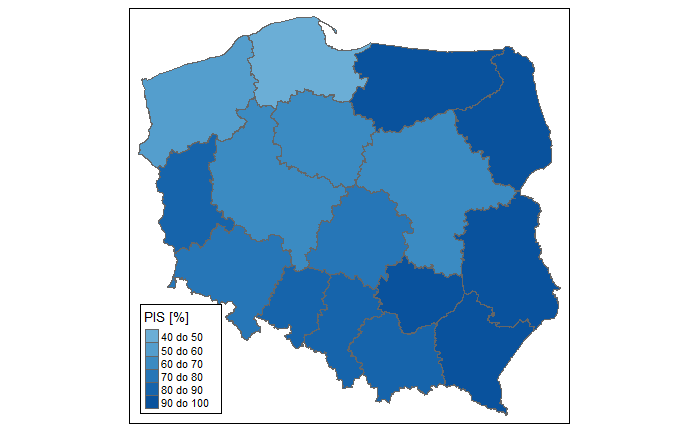
\includegraphics[width=1\textwidth]{rozdzial3/pis_proc_1.jpg}
    \caption{Procentowy podział mandatów KW Prawo i~Sprawiedliwość według województw}
    \caption*{Źródło: opracowanie własne}
    \label{fig:my_label}

    \centering
    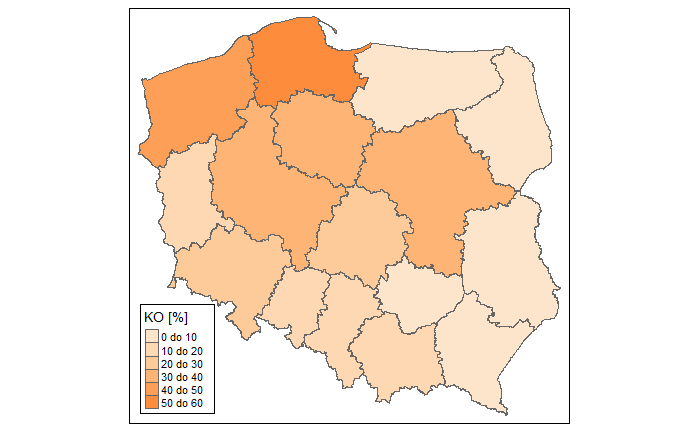
\includegraphics[width=1\textwidth]{rozdzial3/ko_proc_1.jpg}
    \caption{Procentowy podział mandatów KKW Koalicja Obywatelska PO .N IPL Zieloni według województw}
    \caption*{Źródło: opracowanie własne}
    \label{fig:my_label}
\end{figure}



\begin{table}[H]
\caption{Podział mandatów według województw}
\centering
\begin{adjustbox}{angle=90}
\begin{tabular}{l|lllll|lllllll}
\cline{2-13}
 & \multicolumn{5}{c|}{\textbf{Symulacja}} & \multicolumn{7}{c}{\textbf{Wybory do Sejmu RP 2019}} \\ \hline
\textbf{Województwo} & \textbf{PiS} & \textbf{wzrost PiS} & \textbf{KO} & \textbf{wzrost KO} & \textbf{s. mandatów} & \textbf{PiS} & \textbf{KO} & \textbf{SLD} & \textbf{PSL} & \textbf{Konf.} & \textbf{MN} & \textbf{suma} \\
dolnośląskie & 25 & {\color[HTML]{009901} 67\%} & 10 & {\color[HTML]{FE0000} -9\%} & 35 & 15 & 11 & 5 & 2 & 1 &  & 34 \\
kujawsko-pomorskie & 17 & {\color[HTML]{009901} 55\%} & 8 & {\color[HTML]{FFC702} 0\%} & 25 & 11 & 8 & 4 & 2 &  &  & 25 \\
lubelskie & 26 & {\color[HTML]{009901} 53\%} & 0 & {\color[HTML]{FE0000} -100\%} & 26 & 17 & 5 & 2 & 2 & 1 &  & 27 \\
lubuskie & 10 & {\color[HTML]{009901} 150\%} & 2 & {\color[HTML]{FE0000} -50\%} & 12 & 4 & 4 & 2 & 1 & 1 &  & 12 \\
łódzkie & 22 & {\color[HTML]{009901} 29\%} & 9 & {\color[HTML]{009901} 13\%} & 31 & 17 & 8 & 4 & 2 &  &  & 31 \\
małopolskie & 35 & {\color[HTML]{009901} 30\%} & 5 & {\color[HTML]{FE0000} -38\%} & 40 & 27 & 8 & 2 & 3 & 1 &  & 41 \\
mazowieckie i~zagranica & 43 & {\color[HTML]{009901} 30\%} & 21 & {\color[HTML]{009901} 11\%} & 64 & 33 & 19 & 5 & 5 & 1 &  & 63 \\
opolskie & 10 & {\color[HTML]{009901} 100\%} & 2 & {\color[HTML]{FE0000} -50\%} & 12 & 5 & 4 & 1 & 1 &  & 1 & 12 \\
podkarpackie & 25 & {\color[HTML]{009901} 39\%} & 0 & {\color[HTML]{FE0000} -100\%} & 25 & 18 & 4 & 1 & 2 & 1 &  & 26 \\
podlaskie & 14 & {\color[HTML]{009901} 75\%} & 0 & {\color[HTML]{FE0000} -100\%} & 14 & 8 & 3 & 1 & 1 & 1 &  & 14 \\
pomorskie & 13 & {\color[HTML]{009901} 44\%} & 14 & {\color[HTML]{009901} 27\%} & 27 & 9 & 11 & 3 & 1 & 2 &  & 26 \\
śląskie & 47 & {\color[HTML]{009901} 74\%} & 9 & {\color[HTML]{FE0000} -55\%} & 56 & 27 & 20 & 7 &  & 1 &  & 55 \\
świętokrzyskie & 15 & {\color[HTML]{009901} 50\%} & 0 & {\color[HTML]{FE0000} -100\%} & 15 & 10 & 3 & 1 & 1 & 1 &  & 16 \\
warmińsko-mazurskie & 16 & {\color[HTML]{009901} 78\%} & 1 & {\color[HTML]{FE0000} -80\%} & 17 & 9 & 5 & 2 & 2 &  &  & 18 \\
wielkopolskie & 27 & {\color[HTML]{009901} 50\%} & 14 & {\color[HTML]{009901} 8\%} & 41 & 18 & 13 & 6 & 3 &  &  & 40 \\
zachodniopomorskie & 11 & {\color[HTML]{009901} 57\%} & 9 & {\color[HTML]{009901} 13\%} & 20 & 7 & 8 & 3 & 2 &  &  & 20 \\ \hline
\textbf{SUMA} & 356 &  & 104 &  & 460 & 235 & 134 & 49 & 30 & 11 & 1 & 460
\end{tabular}
\end{adjustbox}
\caption*{Źródło: własne}
\end{table}

Jak łatwo można zauważyć według tego scenariusza zmiana ordynacji wyborczej skrajnie dyskryminuje mniejsze komitety, które w~ogóle nie mogłyby wprowadzić żadnego posła do Sejmu. W ten sposób liczą się wyłącznie dwa główne komitety: Prawo i~Sprawiedliwość oraz Koalicja Obywatelska. Jednakowoż Prawo i~Sprawiedliwość i~tak bardzo dużo zyskuje. Znacząco zwiększa liczbę mandatów w~każdym z~województw. Przy czym w~niektórych z~nich zdobywa nawet wszystkie możliwe. Natomiast Koalicja Obywatelska w~znacznej liczbie województw zmniejsza liczbę wygranych mandatów. Wzrost ma głównie w~zachodniej części krajów, która powszechnie jest uważana za bardziej liberalną.

\subsection{Scenariusz II}
Przeprowadzenie prognozy według scenariusza drugiego w~znacznej mierze przebiega analogicznie jak przy scenariuszu pierwszym. Różnicą jest umieszczanie w~tablicy sum głosów oddanych w~danych okręgach nie na dotychczasowe komitety wyborcze, ale na hipotetyczne \enquote{bloki}. Dlatego dodatkowo należało umieścić wzór przypisujący głosy oddane na dotychczasowe komitety według wcześniej ustalonej zasady.

\begin{center}
\begin{table}[H]
\caption{Podział mandatów według Scenariusza II}
\centering
\begin{tabular}{r|l|l}
\centering
\textbf{blok} & \multicolumn{1}{c|}{\textbf{blok lewicowy}} & \multicolumn{1}{c}{\textbf{blok prawicowy}} \\ \hline
\textbf{liczba mandatów} & 211 & 249
\end{tabular}
\caption*{Źródło: własne}
\end{table}
\end{center}


\begin{figure}[H]
    \centering
    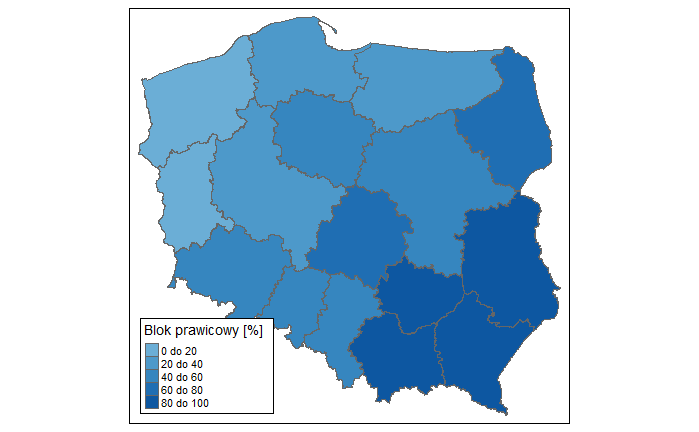
\includegraphics[width=1\textwidth]{rozdzial3/blok_prawicowy_proc.jpg}
    \caption{Procentowy podział mandatów bloku prawicowego według województw}
    \caption*{Źródło: opracowanie własne}
    \label{fig:my_label}

    \centering
    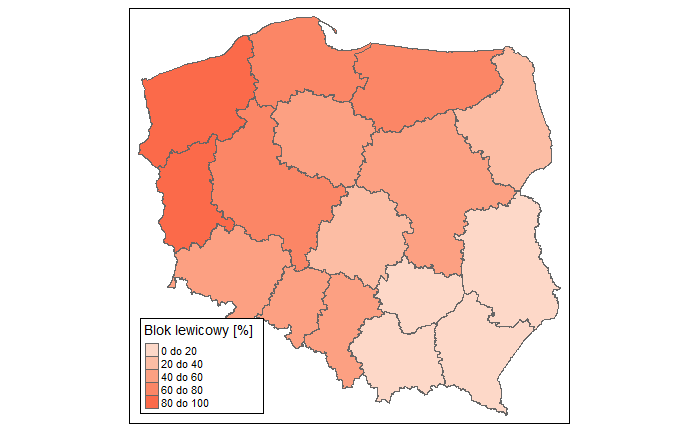
\includegraphics[width=1\textwidth]{rozdzial3/blok_lewicowy_proc.jpg}
    \caption{Procentowy podział mandatów bloku lewicowego według województw}
    \caption*{Źródło: opracowanie własne}
    \label{fig:my_label}
\end{figure}


\begin{table}[H]
\caption{Podział mandatów według województw}
\centering
\scalebox{0.9}{
\begin{tabular}{l|lll}
\cline{2-4}
 & \multicolumn{3}{c}{\textbf{Symulacja}} \\ \hline
\textbf{Województwo} & \textbf{\begin{tabular}[c]{@{}l@{}}blok\\ prawicowy\end{tabular}} & \textbf{\begin{tabular}[c]{@{}l@{}}blok\\ lewicowy\end{tabular}} & \textbf{Suma} \\
dolnośląskie & 18 & 17 & 35 \\
kujawsko-pomorskie & 11 & 14 & 25 \\
lubelskie & 23 & 3 & 26 \\
lubuskie & 1 & 11 & 12 \\
łódzkie & 20 & 11 & 31 \\
małopolskie & 33 & 7 & 40 \\
mazowieckie i~zagranica & 36 & 28 & 64 \\
opolskie & 5 & 7 & 12 \\
podkarpackie & 25 & 0 & 25 \\
podlaskie & 11 & 3 & 14 \\
pomorskie & 6 & 21 & 27 \\
śląskie & 26 & 30 & 56 \\
świętokrzyskie & 14 & 1 & 15 \\
warmińsko-mazurskie & 6 & 11 & 17 \\
wielkopolskie & 13 & 28 & 41 \\
zachodniopomorskie & 1 & 19 & 20 \\ \hline
\textbf{SUMA} & 249 & 211 & 460
\end{tabular}}
\caption*{Źródło: własne}
\end{table}

Wyniki w~tym scenariuszu mocno odbiegają od scenariusza I. Jest to efektem tego, że zakładamy, iż wyborcy mniejszych komitetów poprą blok lewicowy, dzięki czemu przewaga bloku prawicowego, będącego odpowiednikiem Prawa i~Sprawiedliwości, nad blokiem lewicowym zmaleje znacząco. Jedynym województwem, w~którym blok prawicowy zdobywa wszystkie mandaty jest województwo podkarpackie, uważane obecnie za bastion właśnie Prawa i~Sprawiedliwości. Ciekawa zmiana następuje w~województwie lubuskim. W scenariuszu I wygrywa tu Prawo i~Sprawiedliwość zdobywając 11 na 12 mandatów, a~w~scenariuszu II znacząco przegrywa zdobywając tylko 2 na 12 mandatów. Dobrze to pokazuje jak znacząco mogą się zmienić wyniki przy stworzeniu bloków wyborczych łączących wyborców wielu partii oraz, że przy takiej zmianie ordynacji będzie to konieczność dla polskiej sceny politycznej.